% This is samplepaper.tex, a sample chapter demonstrating the
% LLNCS macro package for Springer Computer Science proceedings;
% Version 2.20 of 2017/10/04
%
\documentclass[runningheads]{llncs}
%
\usepackage{graphicx}
% Used for displaying a sample figure. If possible, figure files should
% be included in EPS format.
%
% If you use the hyperref package, please uncomment the following line
% to display URLs in blue roman font according to Springer's eBook style:
% \renewcommand\UrlFont{\color{blue}\rmfamily}

\begin{document}
%
\title{An Event-based Architecture for Multi-population Optimization Algorithms\thanks{Supported by organization x.}}
%
%\titlerunning{Abbreviated paper title}
% If the paper title is too long for the running head, you can set
% an abbreviated paper title here
%
\author{Erick Vargas Minguela\inst{1}\orcidID{0000-1111-2222-3333} \and
Mario Garcia Valdez\inst{2,3}\orcidID{1111-2222-3333-4444} \and
Third Author\inst{3}\orcidID{2222--3333-4444-5555}}
%
\authorrunning{F. Author et al.}
% First names are abbreviated in the running head.
% If there are more than two authors, 'et al.' is used.
%
\institute{National Technological Institute of Mexico 
\email{erick.vargas.minguela@gmail.com}\\
\url{http://www.springer.com/gp/computer-science/lncs}\\
\email{\{abc,lncs\}}}
%
\maketitle              % typeset the header of the contribution
%
\begin{abstract}
    Having the knowledge that both of them are population-based algorithms it can be
    defined that a migration between 2 or more populations are possible, and this kind
    hybrid can be helpful to increase the possibility to find the optimal result (the best
    of the best), there is where fits the concept of Multi-population.
    For this kind of work we used asynchronous functions, serverless functions,
multithread and a distributed architecture taking advantage for functional
programming and serverless architecture.
Even nature works like that... parallel, asynchronous and distributed.

The distributed architectures are having extensive use in the software
industry because of their high performance, many systems are being
created and migrating step by step to microservices and... in a nearly
future... the new architectures called serverless, which proposes the
use of “Function as a Service” (FaaS).

\keywords{Multi-population  \and Asynchronous \and Sub-population \and Serverless \and Distributed.}
\end{abstract}
%
%
%
\section{First Section}
\subsection{A Subsection Sample}
Please note that the first paragraph of a section or subsection is
not indented. The first paragraph that follows a table, figure,
equation etc. does not need an indent, either.

Subsequent paragraphs, however, are indented.

\subsubsection{Sample Heading (Third Level)} Only two levels of
headings should be numbered. Lower level headings remain unnumbered;
they are formatted as run-in headings.

\paragraph{Sample Heading (Fourth Level)}
The contribution should contain no more than four levels of
headings. Table~\ref{tab1} gives a summary of all heading levels.

\begin{table}
\caption{Table captions should be placed above the
tables.}\label{tab1}
\begin{tabular}{|l|l|l|}
\hline
Heading level &  Example & Font size and style\\
\hline
Title (centered) &  {\Large\bfseries Lecture Notes} & 14 point, bold\\
1st-level heading &  {\large\bfseries 1 Introduction} & 12 point, bold\\
2nd-level heading & {\bfseries 2.1 Printing Area} & 10 point, bold\\
3rd-level heading & {\bfseries Run-in Heading in Bold.} Text follows & 10 point, bold\\
4th-level heading & {\itshape Lowest Level Heading.} Text follows & 10 point, italic\\
\hline
\end{tabular}
\end{table}


\noindent Displayed equations are centered and set on a separate
line.
\begin{equation}
x + y = z
\end{equation}
Please try to avoid rasterized images for line-art diagrams and
schemas. Whenever possible, use vector graphics instead (see
Fig.~\ref{fig1}).

\begin{figure}
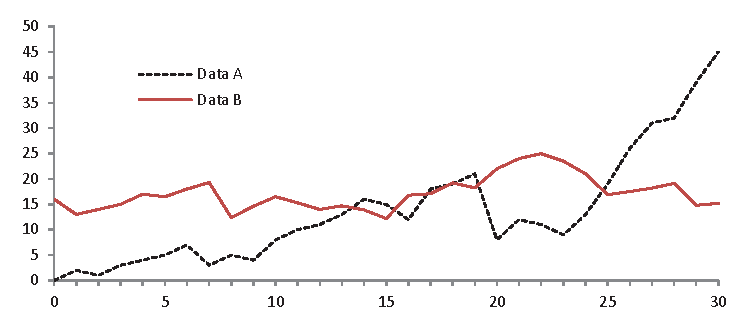
\includegraphics[width=\textwidth]{fig1.eps}
\caption{A figure caption is always placed below the illustration.
Please note that short captions are centered, while long ones are
justified by the macro package automatically.} \label{fig1}
\end{figure}

\begin{theorem}
This is a sample theorem. The run-in heading is set in bold, while
the following text appears in italics. Definitions, lemmas,
propositions, and corollaries are styled the same way.
\end{theorem}
%
% the environments 'definition', 'lemma', 'proposition', 'corollary',
% 'remark', and 'example' are defined in the LLNCS documentclass as well.
%
\begin{proof}
Proofs, examples, and remarks have the initial word in italics,
while the following text appears in normal font.
\end{proof}
For citations of references, we prefer the use of square brackets
and consecutive numbers. Citations using labels or the author/year
convention are also acceptable. The following bibliography provides
a sample reference list with entries for journal
% articles~\cite{ref_article1}, an LNCS chapter~\cite{ref_lncs1}, a
% book~\cite{ref_book1}, proceedings without editors~\cite{ref_proc1},
% and a homepage~\cite{ref_url1}. Multiple citations are grouped
% \cite{ref_article1,ref_lncs1,ref_book1},
% \cite{ref_article1,ref_book1,ref_proc1,ref_url1}.

%-------------------Experiments-----------------------------------------------

\section{Experiments and Results}
\subsection{Experiments}
Now that an interaction between sub-populations with different algorithms it is working and  hybridation have been a success, using until now the added algorithms (GA and PSO) algorithms, all thanks to the 
developed architecture, lets procede to the experiments.
This section is going to be the execution of several experiments from 2 to 40 dimensions, with a stop criterial 
of an error below  0.5E-8, without a parameter optimization method, waiting that the architecture by its self
would be enough to increase the possibility to find a better optimal result than the traditional methods.
All this hoping that the results will probe the needness of this kind of architecture on increasing dimensions.
To test if the architecture was useful, several experiments were made to solve
benchmark functions, for this case the functions are Sphere, Rastrigin and Rosenbrock.
Using 10 sub-population for each experiment and maximum 4 migrations per sub-population with different algorithms and parameters for each sub-population.

\begin{figure}[htp]
    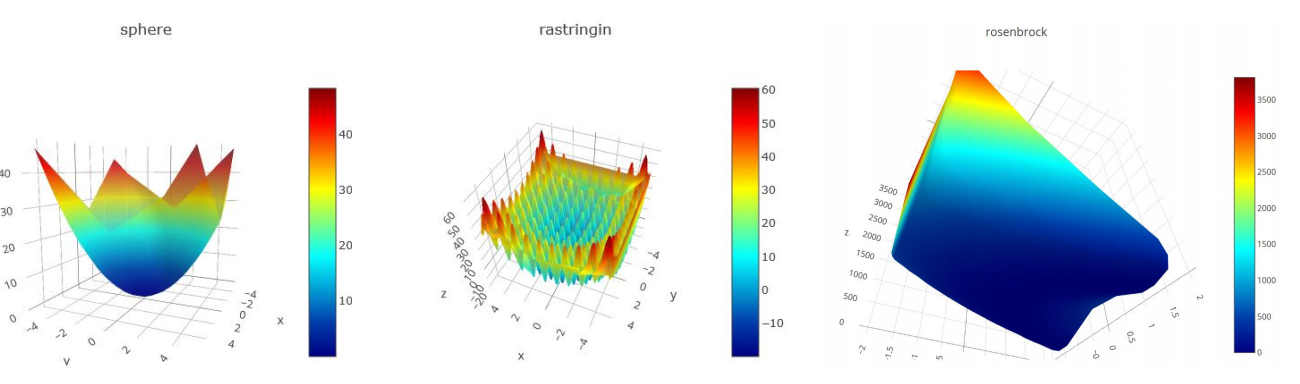
\includegraphics[width=\textwidth]{benchmark.png}
    \caption{Benchmark functions for experimentation.} \label{fig1}
    \end{figure}

\subsection{Parameters Configuration} 

This architecture modifies the traditional way to work with population based algorithms, then the experiments 
could not be parameterized as usually are.

Then the experiments are scaled by their number of evaluations and the
parameters must be configured to be adjusted to the next criterial, using the next expression:

\begin{equation}
    \label{eq:hesitancy-interpretation}
   Evaluations = 10^{5} Dimensions
   \end{equation}











   \begin{table}[htp]
    \caption{Parametros experimentos 2 dimensiones}
    \label{table:ga-pso-parameters-2}
    \centering
    \begin{tabular}{|l|l|}
    \hline
    Parameter & Value \\
    \hline
    \hline
    Optimizaci\'on GA & Minimiza \\
    \hline
    Generaciones GA & 50 \\
    \hline
    Dimensiones GA & 2 \\
    \hline
    Tama\~no de poblaci\'on GA & 100 \\
    \hline
    Mutaci\'on GA & Aleatorio(Tournament2,Tournament3,Random \\
    &  ,RandomLinearRank,Sequential,Fittest)\\
    \hline
    Cruce GA & Tournament3 \\
    \hline
    Porcentaje de cruce GA & Aleatorio[10\%, 80\%] \\
    \hline
    Porcentaje de mutaci\'on GA & Aleatorio[10\%,50\%] \\
    \hline
    Funci\'on de cruce GA & Uniforme de punto medio \\
    \hline
    Funci\'on de mutaci\'on GA & gaussian \\
    \hline
    Optimizaci\'on PSO & Minimiza \\
    \hline
    Iteraciones PSO & 50 \\
    \hline
    Dimensiones PSO & 2 \\
    \hline
    Tama\~no de vector PSO & 100 \\
    \hline
    Factor social PSO & Aleatorio[0.5,4.0] \\
    \hline
    Factor individual PSO & Aleatorio[0.5,4.0] \\
    \hline
    Peso de inercia PSO & Aleatorio[0.5,4.0] \\
    \hline
    \end{tabular}
    \end{table}

\begin{figure}[htp]
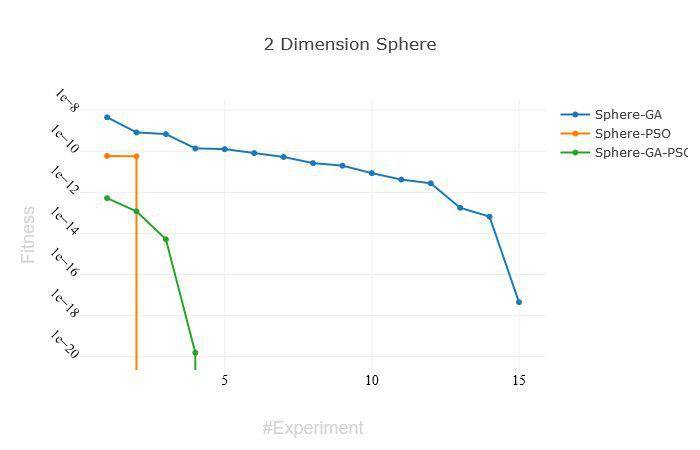
\includegraphics[width=\textwidth]{2-sphere.jpg}
\caption{Benchmark functions for experimentation.} \label{fig1}
\end{figure}

\begin{table}[htp]
    \caption{Resultados 2 dimensiones}
    \label{table:resultados-2}
    \centering
    \begin{tabular}{|c|c|c|c|}
    \hline
    Fn & Mejor & Promedio & No. Experimento \\
    \hline
    \hline
    Rastrigin GA & 0 & 1.65377E-08 & 15\\
    \hline
    Rastrigin PSO & 0 & 1.8872E-12 & 15\\
    \hline
    Rastrigin GA-PSO & 0 & 0 & 15\\
    \hline
    Sphere GA & 4.53222E-18 & 4.36977E-10 & 15\\
    \hline
    Sphere PSO & 0 & 7.8012E-12 & 15\\
    \hline
    Sphere GA-PSO & 0 & 4.33161E-14 & 15\\
    \hline
    Rosenbrock GA & 1.62335E-13 & 1.24176E-08 & 15\\
    \hline
    Rosenbrock PSO & 1.11674E-12 & 2.47795E-06 & 15\\
    \hline
    Rosenbrock GA-PSO & 9.5809E-14 & 6.90695E-09 & 15\\
    \hline
    \end{tabular}
    \end{table}
  

% ---- Bibliography ----
%
% BibTeX users should specify bibliography style 'splncs04'.
% References will then be sorted and formatted in the correct style.
%
% \bibliographystyle{splncs04}
% \bibliography{mybibliography}
%


   \begin{thebibliography}{10}

    \bibitem{Hellerstein2018}
    J.~M. Hellerstein, J.~Faleiro, J.~E. Gonzalez, J.~Schleier-Smith, V.~Sreekanti,
      A.~Tumanov, and C.~Wu, ``{Serverless Computing: One Step Forward, Two Steps
      Back},'' vol.~3, 2018.
    
    \bibitem{Kramer2017}
    O.~Kramer, ``{Genetic Algorithm Essentials},'' {\em Springer International
      Publishing AG}, vol.~679, pp.~11--20, 2017.
    
    \bibitem{Guerrero2017}
    C.~Guerrero, I.~Lera, and C.~Juiz, ``{Genetic Algorithm for Multi-Objective
      Optimization of Container Allocation in Cloud Architecture},'' {\em Journal
      of Grid Computing}, pp.~1--23, 2017.
    
    \bibitem{Lalwani2019}
    S.~Lalwani, H.~Sharma, S.~Chandra, S.~Kusum, D.~Jagdish, and C.~Bansal,
      ``{REVIEW - COMPUTER ENGINEERING AND COMPUTER SCIENCE A Survey on Parallel
      Particle Swarm Optimization Algorithms},'' {\em Arabian Journal for Science
      and Engineering}, 2019.
    
    \bibitem{Blum2005}
    S.~Blum, R.~Puisa, and M.~Wintermantel, ``{Adaptive Mutation Strategies for
      Evolutionary Algorithms},'' {\em 2nd Weimar Optimization and Stochastic
      Days}, pp.~1--13, 2005.
    
    \bibitem{Everywhere}
    S.~Everywhere, ``{The Fn Project},''
    
    \bibitem{Ma2019}
    H.~Ma, S.~Shen, M.~Yu, Z.~Yang, M.~Fei, and H.~Zhou, ``{Multi-population
      techniques in nature inspired optimization algorithms : A comprehensive
      survey},'' {\em Swarm and Evolutionary Computation}, vol.~44, no.~July 2017,
      pp.~365--387, 2019.
    
    \bibitem{Santander-jim2018}
    S.~Santander-jim and M.~A. Vega-rodr, ``{Comparative Analysis of
      Intra-Algorithm Parallel Multiobjective Evolutionary Algorithms : Taxonomy
      Implications on Bioinformatics Scenarios},'' vol.~9219, no.~c, pp.~1--15,
      2018.
    
    \bibitem{Sherry2012}
    D.~Sherry, K.~Veeramachaneni, J.~McDermott, and U.~M. O'Reilly, ``{Flex-GP:
      Genetic programming on the cloud},'' {\em Lecture Notes in Computer Science
      (including subseries Lecture Notes in Artificial Intelligence and Lecture
      Notes in Bioinformatics)}, vol.~7248 LNCS, pp.~477--486, 2012.
    
    \bibitem{Goebel2016}
    R.~Goebel, {\em {29th Australasian Joint Conference on Artificial Intelligence,
      AI 2016}}, vol.~9992 LNAI.
    \newblock 2016.
    
    \bibitem{Guerv2018}
    J.~J.~M. Guerv and J.~M. Garc, ``{Introducing an Event-Based Architecture for
      Concurrent and Distributed Evolutionary Algorithms},'' vol.~1, pp.~399--410,
      2018.
    
    \bibitem{Moroney2017}
    L.~Moroney, {\em {The Definitive Guide to Firebase: Build Android Apps on
      Google's Mobile Platform}}.
    \newblock 2017.
    
    \bibitem{Ambler2015}
    T.~Ambler and N.~Cloud, {\em {JavaScript frameworks for modern web dev}}.
    \newblock 2015.
    
    \bibitem{Barwell2016}
    A.~D. Barwell, C.~Brown, and K.~Hammond, ``{USING PROGRAM SHAPING AND
      ALGORITHMIC SKELETONS TO PARALLELISE AN EVOLUTIONARY MULTI-AGENT SYSTEM IN
      ERLANG Wojciech Turek , Aleksander Byrski},'' vol.~35, pp.~792--818, 2016.
    
    \bibitem{Paper2017}
    C.~Paper and E.~Alba, ``{Distributed Genetic Algorithms on Portable Devices for
      Smart Cities},'' no.~May, 2017.
    
    \bibitem{Technische2016}
    J.~L. Technische, ``{C6.3 Island (migration) models: evolutionary algorithms
      based on punctuated equilibria},'' no.~January 2000, 2016.
    
    \bibitem{Kunasaikaran2016}
    J.~Kunasaikaran and A.~Iqbal, ``{A Brief Overview of Functional Programming
      Languages},'' {\em electronic Journal of Computer Science and Information
      Technology (eJCSIT)}, vol.~6, no.~1, pp.~32--36, 2016.
    
    \bibitem{Hows2014}
    D.~Hows, P.~Membrey, and E.~Plugge, ``{MongoDB Basics},'' {\em MongoDB Basics},
      2014.
    
    \bibitem{Cook2017}
    J.~Cook, {\em {Docker for Data Science}}.
    \newblock 2017.
    
    \bibitem{Lovbjerg2001}
    M.~L{\o}vbjerg and T.~K. Rasmussen, ``{Hybrid Particle Swarm Optimiser with
      Breeding and Subpopulations},'' {\em Proc. 3rd Genetic Evolutionary
      Computation Conf.}, pp.~469 --476, 2001.
    
    \bibitem{Jimeno2019}
    H.~M.~A. Jimeno, M.~J.~L. S{\'{a}}nchez, and R.~H. Rico, ``{Multipopulation ‑
      based multi ‑ level parallel enhanced Jaya algorithms},'' {\em The Journal
      of Supercomputing}, no.~0123456789, 2019.
    
    \bibitem{Roberts2016}
    M.~Roberts, ``{Serverless Architectures},'' 2016.
    
    \bibitem{Kaya2011}
    Y.~Kaya, M.~Uyar, and R.~Tek$\backslash$D{\{}j{\}}n, ``{A Novel Crossover
      Operator for Genetic Algorithms: Ring Crossover},'' no.~May 2014, 2011.
    
    \end{thebibliography}
\end{document}
